%\documentclass[12pt,a4paper,addpoints]{exam}
\documentclass[12pt,a4paper,addpoints,answers]{exam}
\usepackage[T1]{fontenc}
\usepackage[utf8]{inputenc}
\usepackage[spanish]{babel}
\usepackage{multirow}
\usepackage{graphicx}
\usepackage{xcolor}
\usepackage{listings}
\usepackage{upquote}
\usepackage{xcolor}
\usepackage{listings}
\usepackage{amsmath}


% Definición de colores
\definecolor{keywordcolor}{rgb}{0.1,0.1,0.8} % Azul para palabras clave
\definecolor{stringcolor}{rgb}{0.8,0.1,0.1}  % Rojo para cadenas
\definecolor{commentcolor}{rgb}{0.1,0.6,0.1} % Verde para comentarios

% Configuración de listings
\lstdefinestyle{mysqlstyle}{
  basicstyle=\ttfamily\footnotesize,          % Estilo básico
  keywordstyle=\color{keywordcolor}\bfseries, % Estilo para palabras clave
  commentstyle=\color{commentcolor}\itshape,  % Estilo para comentarios
  stringstyle=\color{stringcolor},            % Estilo para cadenas
  showstringspaces=false,                     % No mostrar espacios en cadenas
  tabsize=2,                                  % Tamaño de tabulación
  breaklines=true,                            % Dividir líneas largas
  morestring=[b]",                            % Cadenas con comillas dobles
  literate={ñ}{{\~n}}1,                       % Permite el carácter "ñ"
  morekeywords={SELECT, INSERT, UPDATE, DELETE, FROM, WHERE, JOIN, INNER, LEFT, RIGHT, ON, GROUP, BY, ORDER, ASC, DESC, CREATE, TABLE, DROP, ALTER, DATABASE, USE, INDEX, INTO, VALUES, SET, IF, EXISTS, NOT, NULL, AND, HAVING, COUNT, DISTINCT, LIKE, BEFORE, FOR, EACH, ROW, DECLARE, IF, SIGNAL, OPEN, CURSOR, FOUND, USER, TO, IDENTIFIED} % Palabras clave SQL
}

% Usar el estilo
\lstset{style=mysqlstyle}



% Términos en castellano
\pointpoints{Punto}{Puntos}
\renewcommand{\solutiontitle}{\noindent\textbf{Solución propuesta:}\enspace\\}
\renewcommand{\questionlabel}{\textbf{EJERCICIO \thequestion.}}

% Tabla para que el alumno introduzca sus datos
\def\studentdata{
    \begin{table}[t]
        \renewcommand{\arraystretch}{1.2}
        \small
        \centering
        \begin{tabular}{|l|p{4cm}|p{4cm}|p{2.5cm}|}
            \hline
            \multirow{3}{*}{
\includegraphics[width=2.5cm]{logos/etsisi.png}} & \multicolumn{3}{l|}{Apellidos:} \\ \cline{2-4} 
                                                                             & \multicolumn{3}{l|}{Nombre:}    \\ \cline{2-4} 
                                                                             & DNI:  & Num. mat.: & Grupo: \\ \hline
        \end{tabular}%
    \end{table}
}

% Estilo de la cabecera y pie de pagina
\pagestyle{headandfoot}
\firstpageheadrule
\runningheadrule
\header{Bases de Datos}{}{Convocatoria ordinaria\\Curso 2024/2054}
\firstpagefootrule
\runningfootrule
\footer{}{}{Página\,\thepage\,de\,\numpages}

\begin{document}

\studentdata

\begin{center}\textbf{Normativa de examen}\end{center}
\begin{itemize}
    \item No está permitido el uso de dispositivos móviles ni otros dispositivos electrónicos, así como libros ni apuntes.
    \item Durante el examen, los profesores podrán solicitar acreditar la identidad de los participantes en el mismo. Deberá tener en todo momento su Documento Nacional de Identidad y/o Carné de la Universidad Politécnica de Madrid visible sobre la mesa.
    \item Deberá escribir su nombre, con bolígrafo, en todas las hojas de las que consta el examen.
    \item Los ejercicios deberán resolverse con bolígrafo, excepto el diagrama solicitado en el ejercicio 1, el cual podrá completarse opcionalmente a lápiz.
    \item No se permite abandonar el aula de examen durante los primeros 20 minutos. Transcurrido este tiempo, no se permitirá entrar al examen. 
    \item El examen tiene una duración máxima de \textbf{2 horas y 30 minutos}. 
    \item Justifique sus respuestas lo mejor posible indicando, si fuese necesario, los pasos realizados.
    \item Las calificaciones provisionales serán publicadas en el Moodle de la asignatura a los 15 días hábiles desde la fecha de realización del examen.
    \item La fecha para la revisión del examen se anunciará en el Moodle de la asignatura una vez publicadas las calificaciones provisionales.
\end{itemize}
\newpage

\begin{questions}

\question[2\half] Modelado entidad relación

Realizar un modelo conceptual de datos mediante la técnica del modelo \textbf{Entidad Relación de Chen} teniendo en cuenta la siguiente descripción:

\begin{quotation}
A la vista de la catástrofe ocurrida el 29 de octubre de 2024 en Valencia y Albacete a raíz de una DANA, la organización CUPAS (Coordinémonos Un Poco Aunque Sea) desea crear una base de datos que permita gestionar de manera eficiente los recursos, servicios y personal movilizado para atender cualquier posible situación de emergencia futura. Para ello, se proponen diseñar una base de datos que permita almacenar y gestionar la información de los servicios de emergencia, los equipos de voluntarios y las máquinas y vehículos utilizados.

En cuanto a los servicios de emergencia, el sistema debe almacenar información sobre los distintos servicios existentes (bomberos, policía, protección civil, ambulancias, etcétera). De cada servicio de emergencia es imprescindible almacenar el tipo de servicio (por ejemplo: ``bomberos'' o ``ambulancia''), el origen (por ejemplo: ``Parque Bomberos PB-12 (Madrid)''), el número de personal movilizado y el contacto del responsable del servicio. Además, cada servicio dispondrá de vehículos y/o máquinas que también deberán quedar registrados. Con respecto a las máquinas, será necesario almacenar su código, nombre, y estado (operativo o no operativo). Asimismo, de los vehículos se debe registrar su matrícula, tipo (por ejemplo: camión de bomberos, ambulancia, tractor), estado (operativo o no operativo) y kilometraje actual. Las máquinas y vehículos de cada servicio de emergencias se podrán emplear únicamente mientras dicho servicio esté actuando en la catástrofe.

Por otro lado, la base de datos también debe poder almacenar información relativa a los voluntarios, que estarán organizados en equipos liderados por un coordinador. Cada equipo se identificará por un nombre único y podrá desarrollar tareas de un único tipo (por ejemplo: limpieza, búsqueda de víctimas, suministro de alimentos, etcétera). Por otra parte, de cada voluntario, que se identificará por su documento de identidad, se debe almacenar su nombre y apellidos y el teléfono. Es posible que los voluntarios cambien de equipo dependiendo de las necesidades de cada día.

Tanto los servicios de emergencias como los equipos de voluntarios serán asignados a tareas (por ejemplo: rescate de víctimas, remolcado de vehículos, desescombro, extracción de lodo, limpieza de calles, suministro de alimentos, etcétera), que dispondrán de un identificador único. En cada tarea puede participar uno o más equipos o servicios de emergencia, y puede suceder que durante la realización de la tarea comiencen a trabajar nuevos equipos o dejen de trabajar equipos existentes, por lo que será necesario almacenar la fecha de inicio y de fin en la que cada servicio de emergencia o equipo de voluntarios comienza a trabajar en ellas. Además, en el caso de los servicios de emergencias, se les puede asignar varias tareas a la vez. Por último, también será necesario almacenar la fecha de inicio y la fecha de fin de cada tarea, así como una descripción de la misma y la localidad en la que se desarrolla.
\end{quotation}

Se pide realizar un \textbf{modelo entidad-relación de Chen} justificando las cardinalidades mínimas de al menos dos relaciones \textbf{cardinalidades mínimas}.

\begin{solution}[50em]
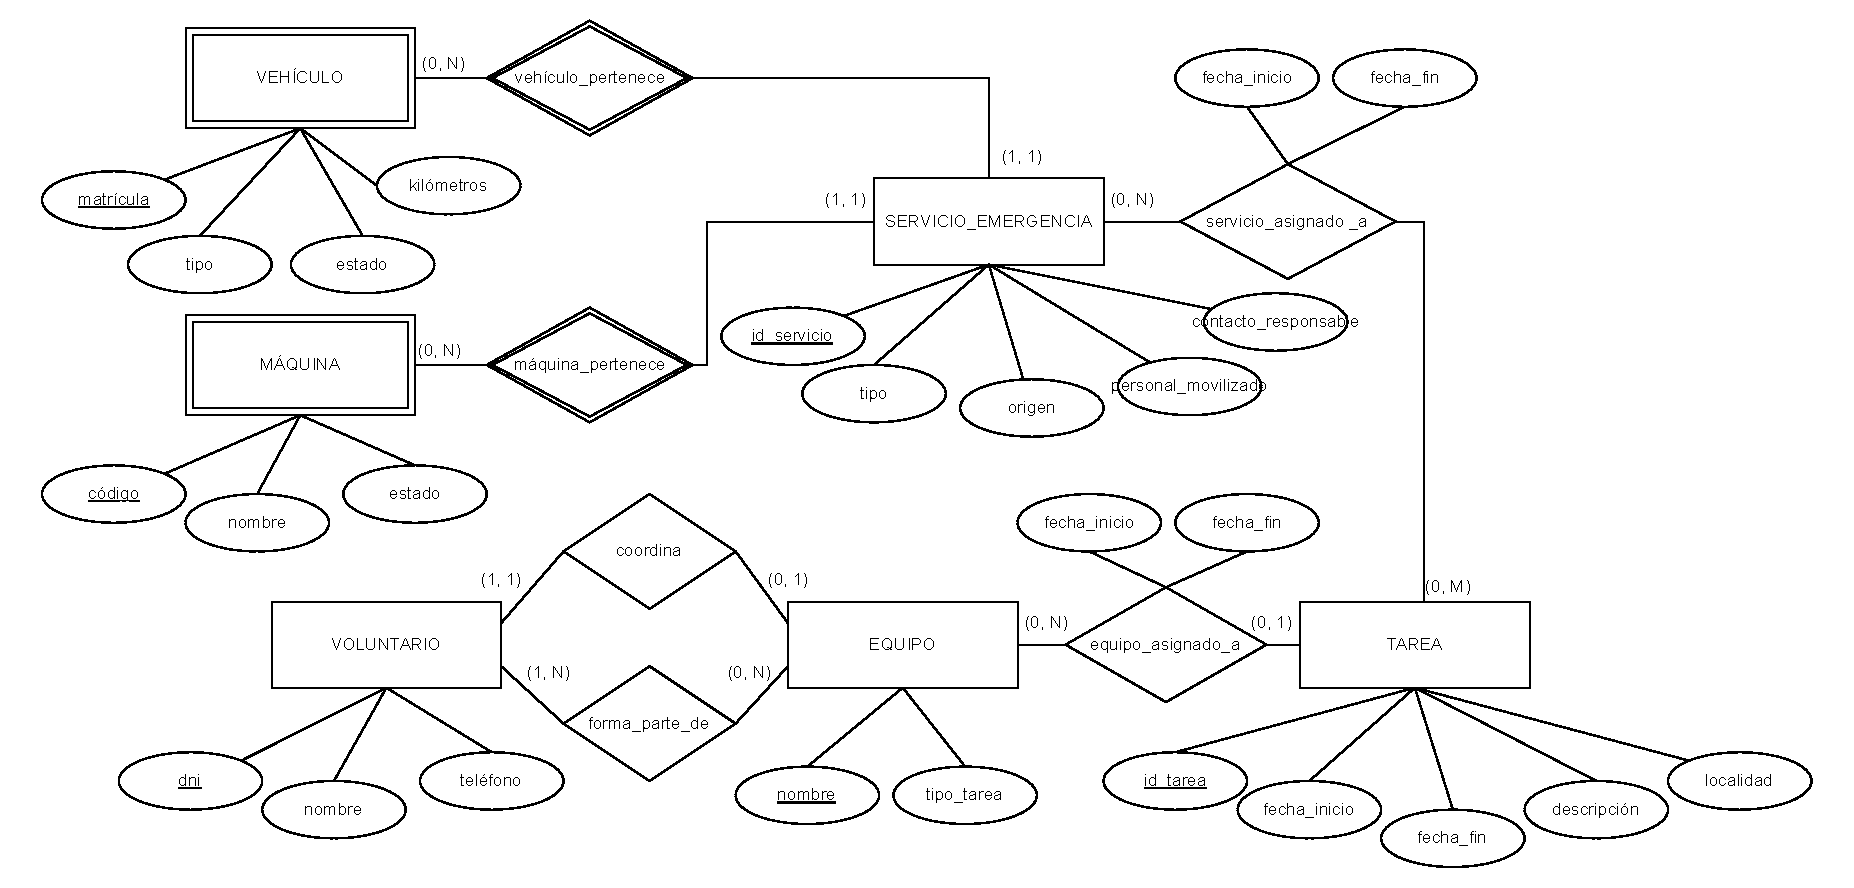
\includegraphics[width=\textwidth]{figs/bbdd-2024-2025-ordinaria/MER.pdf}

Cardinalidades mínimas:
\begin{itemize}
    \item La cardinalidad mínima de máquina con respecto a servicio de emergencias es 0, ya que un servicio de emergencias puede tener o no máquinas. Por otro lado, la cardinalidad mínima de servicio de emergencias es 1, puesto que si existe una máquina, debe pertenecer a un servicio de emergencias.
    \item La cardinalidad mínima de servicio de emergencias con tarea es 0, ya que un servicio de emergencias puede existir sin que se le haya asignado todavía ninguna tarea. Por otra parte, la cardinalidad mínima de tarea con respecto a servicio de emergencias es 0, puesto que puede existir una tarea a la que no se le haya asignado ningún equipo de emergencias.
\end{itemize}
\end{solution}

\newpage
\question Dado el siguiente modelo relacional\footnote{Tenga en cuenta que las claves primarias aparecen \underline{subrayadas} mientras que las claves foráneas aparece en \textit{cursiva} junto con el superíndice \textsuperscript{FK} y comparten nombre con la clave primaria a la que referencian.} que representa la base de datos de una empresa de gestión de centros comerciales:

\texttt{CENTRO\_COMERCIAL (\underline{idCentroComercial}, nombre, calle, número, municipio)}

\texttt{TIENDA (\underline{idTienda}, nombre, \textit{idCentroComercial\textsuperscript{FK}}, \textit{idCategoria\textsuperscript{FK}}, local)}

\texttt{CATEGORÍA (\underline{idCategoria}, nombre)}

\texttt{COMPRA (\underline{\textit{idCliente\textsuperscript{FK}}}, \underline{\textit{idTienda\textsuperscript{FK}}}, cantidad, \underline{día}, \underline{mes}, \underline{año})}

\texttt{CLIENTE (\underline{idCliente}, nombre, apellidos, municipio)}

% Añadido para hibernate
\texttt{TRABAJA (\underline{\textit{idEmpleado\textsuperscript{FK}}}, \underline{\textit{idTienda\textsuperscript{FK}})}}

\texttt{EMPLEADO (\underline{idEmpleado}, nombre, apellidos, edad, sueldo)}

Se pide dar respuesta a las siguientes cuestiones:

\begin{parts}
\part[\half] Resuelva con álgebra relacional la siguiente consulta: ``\textit{nombres y municipios de los centros comerciales que no vendieron nada durante el mes de abril del año 2020}''.
\begin{solution}[20em]

$\Pi_{nombre,municipio}(CENTRO\_COMERCIAL) \bowtie ($

$\quad \Pi_{idCentroComercial} (CENTRO\_COMERCIAL)$

$\quad -$

$\quad \Pi_{idCentroComercial} (TIENDA \bowtie \sigma_{\text{mes=4 \& año=2020}} (COMPRA))$

$)$
\end{solution}

\part[\half] Resuelva con álgebra relacional la siguiente consulta: ``\textit{nombres y municipios de los centros comerciales con tiendas de todas las categorías}''.
\begin{solution}[20em]

$\Pi_{nombre,municipio}(CENTRO\_COMERCIAL \bowtie ($

$\quad \Pi_{idCentroComercial, idCategoria} (TIENDA) \div \Pi_{idCategoria} (CATEGORIA)$

$))$
\end{solution}

\newpage
\part[\half] Resuelva mediante SQL la siguiente consulta: ``\textit{nombre y apellidos del cliente o clientes que más han gastado en los centros comerciales del municipio de Madrid}''.
\begin{solution}[20em]
\begin{lstlisting}[language=SQL]
SELECT cliente.nombre, cliente.apellidos
FROM cliente
  INNER JOIN compra 
    ON compra.idCliente = cliente.idCliente
  INNER JOIN tienda 
    ON tienda.idTienda = compra.idTienda
  INNER JOIN centro_comercial cc
    ON cc.idCentroComercial = tienda.idCentroComercial
WHERE cc.municipio = 'Madrid'
GROUP BY cliente.idCliente, cliente.nombre, cliente.apellidos
HAVING SUM(cantidad) 
    >= ALL (SELECT SUM(cantidad)
            FROM compra
              INNER JOIN tienda 
                ON tienda.idTienda = compra.idTienda
              INNER JOIN centro_comercial cc
                ON cc.idCentroComercial = tienda.idCentroComercial
            WHERE municipio = 'Madrid'
            GROUP BY idCliente)

\end{lstlisting}
\end{solution}

\part[\half] Resuelva mediante SQL la siguiente consulta: ``\textit{nombre y apellidos de los clientes que nunca han comprado en un centro comercial fuera de su municipio}''.
\begin{solution}[20em]
\begin{lstlisting}[language=SQL]
SELECT nombre, apellidos
FROM cliente
WHERE idCliente NOT IN 
  (SELECT idCliente
   FROM cliente
     INNER JOIN compra ON compra.idCliente = cliente.idCliente
     INNER JOIN tienda ON tienda.idTienda = compra.idTienda
     INNER JOIN centro_comercial cc ON cc.idCentroComercial = tienda.idCentroComercial
   WHERE cliente.idCliente = compra.idCliente
     AND cliente.municipio <> cc.municipio)
\end{lstlisting}
\end{solution}

\newpage
\part[\half] Resuelva mediante SQL la siguiente consulta: ``\textit{nombre y apellidos de los clientes que han comprado en todas las tiendas de la segunda planta del centro comercial con identificador 16 (i.e.  \texttt{idCentroComercial = 16}). Las tiendas de la segunda planta son aquellas cuyo local comienza por la cadena \texttt{`L2-'}}''.
\begin{solution}[20em]
\begin{lstlisting}[language=SQL]
SELECT cliente.nombre, cliente.apellidos
FROM compra 
  INNER JOIN tienda ON tienda.idTienda = compra.idTienda
  INNER JOIN cliente ON cliente.idCliente = compra.idCliente
WHERE idCentroComercial = 16
  AND local LIKE 'L2-%'
GROUP BY cliente.idCliente, cliente.nombre, cliente.apellidos
HAVING COUNT(DISTINCT tienda.idTienda) = (SELECT COUNT(*)
                                          FROM tienda
                                          WHERE idCentroComercial = 16
                                            AND local LIKE 'L2-%')
\end{lstlisting}
\end{solution}

\part[\half] Resuelva mediante SQL la siguiente consulta: ``\textit{nombre y apellidos de los empleados que han trabajado tanto en tiendas de la categoría denominada `hogar' como en tiendas de la categoría denominada `deportes' }''.
\begin{solution}[20em]
\begin{lstlisting}[language=SQL]
SELECT nombre, apellidos
FROM empleado
WHERE idEmpleado IN (SELECT idEmpleado
                     FROM trabaja
                        NATURAL JOIN cetegoria
                     WHERE nombre = 'hogar')
  AND idEmpleado IN (SELECT idEmpleado
                     FROM trabaja
                        NATURAL JOIN cetegoria
                     WHERE nombre = 'deportes')
\end{lstlisting}
\end{solution}

\newpage
\part[\half] Escriba una sentencia en SQL que permita borrar todos los centros comerciales que hayan facturado menos de 1.000.000 durante el año 2024.
\begin{solution}[20em]
\begin{lstlisting}[language=SQL]
DELETE FROM centro_comercial
WHERE idCentroComercial IN (SELECT idCentroComercial
                            FROM tienda
                              INNER JOIN compra ON compra.idTienda = tienda.idTienda
                            WHERE año = 2024
                            GROUP BY idCentroComercial
                            HAVING SUM(cantidad) < 1000000);
\end{lstlisting}\end{solution}
\end{parts}

\newpage
\question Basándonos en la base de datos del modelo relacional propuesto en el ejercicio 2.

\begin{parts}
\part[1] Escribir un \emph{PROCEDIMIENTO} que calcule el desglose mensual de las cantidades totales vendidas por las tiendas de un centro comercial específico durante un año determinado. El resultado se debe devolver en un parámetro de salida que será una cadena de texto donde, para cada mes del año, se indique la cantidad total vendida por las tiendas del centro comercial, siguiendo el formato: `\texttt{Mes1:300|Mes2:450|...|Mes12:500}'. Será obligatorio el uso de un \texttt{CURSOR} para implementar este procedimiento, y se puede utilizar la función \texttt{CONCAT}\footnote{La función \texttt{CONCAT} permite concatenar varias cadenas de texto. Por ejemplo, \texttt{CONCAT(`a',`b',`c')} devuelve la cadena \texttt{`abc'}.} para concatenar las cadenas que formen el texto de salida.

\begin{solution}[52em]
\begin{lstlisting}[language=SQL]
DELIMITER $$
CREATE PROCEDURE ventasMensualesPorCentroComercial (IN idCC INTEGER, IN anio INTEGER, OUT resultado VARCHAR(256))
BEGIN
    DECLARE mes, cantidad INTEGER;
    DECLARE primermes INT DEFAULT TRUE;
    DECLARE done INT DEFAULT FALSE;
    DECLARE cur1 CURSOR FOR SELECT mes, SUM(co.cantidad)
                            FROM compra co 
                              INNER JOIN tienda t 
                                ON co.idTienda = t.idTienda 
                            WHERE cc.idCentroComercial = idCC 
                              AND co.año = anio
                            GROUP BY mes
                            ORDER BY mes;
    DECLARE CONTINUE HANDLER FOR NOT FOUND SET done = TRUE;
    
    OPEN cur1;
    read_loop: LOOP
        FETCH cur1 INTO mes, cantidad;
        IF done THEN
            LEAVE read_loop;
        END IF;

        IF primermes THEN
            SET resultado = CONCAT('Mes',mes,':',cantidad); 
            primermes = FALSE;
        ELSE
            SET resultado = CONCAT(resultado, '|', 'Mes',mes,':',cantidad);
        END IF;
    END LOOP;
    CLOSE cur1;
END$$
DELIMITER ;

\end{lstlisting}        
\end{solution}

\newpage
\part[1] Se quiere evitar la creación de monopolios dentro de los centros comerciales, es decir que una categoría de tipo de tiendas se convierta en dominante dentro de un centro comercial. Para ello se debe escribir un \emph{TRIGGER} que al dar de alta nuevas tiendas no permita que el porcentaje de tiendas de una misma categoría supere un umbral del 10\% del total de tiendas en el centro comercial en el que se encuentra dicha tienda.
\begin{solution}
\begin{lstlisting}[language=SQL]

DELIMITER $$
CREATE TRIGGER verificarMonopolioDeCategoria AFTER INSERT ON tienda
FOR EACH ROW
BEGIN
    DECLARE totalTiendasEnCentro INT;
    DECLARE totalTiendasCategoria INT;
    DECLARE porcentajeCategoria DECIMAL(5, 2);

    SELECT COUNT(*) INTO totalTiendasEnCentro
    FROM tienda
    WHERE idCentroComercial = NEW.idCentroComercial;

    SELECT COUNT(*) INTO totalTiendasCategoria
    FROM tienda
    WHERE idCentroComercial = NEW.idCentroComercial
      AND idCategoria = NEW.idCategoria;

    SET porcentajeCategoria = (totalTiendasCategoria / totalTiendasEnCentro) * 100;

    IF porcentajeCategoria > 10 THEN
        SIGNAL SQLSTATE '02000'
        SET MESSAGE_TEXT = 'No se puede insertar la tienda. El porcentaje de tiendas de esta categoria excede el limite del centro comercial';
    END IF;
END$$
DELIMITER ;

\end{lstlisting}       
\end{solution}
\end{parts}

\newpage
\studentdata
\question[\half] Con base en la base de datos del modelo relacional propuesto en el ejercicio 2, se requiere mejorar la seguridad implementando controles de acceso a la tabla \texttt{empleado}. El objetivo es garantizar que únicamente un nuevo usuario, identificado como \texttt{recursos\_humanos}, tenga permiso para realizar operaciones de lectura y escritura (inserción, actualización y eliminación) sobre esta tabla.

Se solicita detallar todas las sentencias SQL necesarias para:
\begin{enumerate}
    \item Crear el usuario \texttt{recursos\_humanos}.
    \item Asignarle permisos específicos de lectura y escritura sobre la tabla empleado.
\end{enumerate}


\begin{solution}
\begin{lstlisting}[language=SQL]
CREATE USER 'recursos_humanos' IDENTIFIED BY 'password';

GRANT SELECT, INSERT, UPDATE, DELETE ON EMPLEADO TO 'recursos_humanos';

\end{lstlisting}       
\end{solution}

\newpage
\question[1] A partir de la base de datos relacional propuesta en el ejercicio 2, complete el esqueleto de código proporcionado a continuación añadiendo las anotaciones necesarias para implementar las relaciones entre las entidades \texttt{CENTRO\_COMERCIAL}, \texttt{TIENDA}, \texttt{EMPLEADO} y \texttt{TRABAJO}, utilizando el lenguaje \texttt{Java} y la librería \texttt{Hibernate}.

\begin{lstlisting}[language=Java]



public class CentroComercial {

    
    
    private Integer idCentroComercial;


    
    private String nombre;


    
    private String calle;


    
    private String numero;


    
    private String municipio;


    
    private List<Tienda> tiendas = new ArrayList<>();

    // Getters y setters
}



public class Tienda {


    
    private Integer idTienda;


    
    private String nombre;


    
    private CentroComercial centroComercial;


    
    private String local;


    
    private List<Empleado> empleados = new ArrayList<>();

    // Getters y setters
}



public class Empleado {


    
    private Integer idEmpleado;


    
    private String nombre;


    
    private String apellidos;


    
    private Integer edad;


    
    private String sueldo;


    
    private List<Tienda> tiendas = new ArrayList<>();

    // Getters y setters
}
\end{lstlisting} 


\begin{solution}
\begin{lstlisting}[language=Java]
@Entity
@Table(name = "CENTRO_COMERCIAL")
public class CentroComercial {

    @Id
    @GeneratedValue
    @Column(name = "idCentroComercial")
    private Integer idCentroComercial;

    @Column(name = "nombre", nullable = false)
    private String nombre;

    @Column(name = "calle", nullable = false)
    private String calle;

    @Column(name = "numero")
    private String numero;

    @Column(name = "municipio")
    private String municipio;

    @OneToMany(mappedBy = "centroComercial", cascade = CascadeType.ALL)
    private List<Tienda> tiendas = new ArrayList<>();

    // Getters y setters
}

@Entity
@Table(name = "TIENDA")
public class Tienda {

    @Id
    @GeneratedValue
    @Column(name = "idTienda")
    private Integer idTienda;

    @Column(name = "nombre", nullable = false)
    private String nombre;

    @ManyToOne
    @JoinColumn(name = "idCentroComercial", nullable = false)
    private CentroComercial centroComercial;

    @Column(name = "local")
    private String local;

    @ManyToMany(mappedBy = "tiendas")
    private List<Empleado> empleados = new ArrayList<>();

    // Getters y setters
}

@Table(name = "EMPLEADO")
public class Empleado {

    @Id
    @GeneratedValue
    @Column(name = "idEmpleado")
    private Integer idEmpleado;

    @Column(name = "nombre", nullable = false)
    private String nombre;

    @Column(name = "apellidos", nullable = false)
    private String apellidos;

    @Column(name = "edad")
    private Integer edad;

    @Column(name = "sueldo")
    private String sueldo;

    @ManyToMany()
    @JoinTable(name = "TRABAJA")
    private List<Tienda> tiendas = new ArrayList<>();

    // Getters y setters
}
\end{lstlisting}       
\end{solution}

\newpage
\question[\half] Basándonos en la base de datos del modelo relacional propuesto en el ejercicio 2, se han creado las siguientes tablas con sus respectivos valores. Se pide generar \textbf{un único documento JSON embebido} tomando como raíz principal \texttt{centros\_comerciales}, y manteniendo toda la información que aparece en las tablas.

% Tabla CENTRO_COMERCIAL
\begin{table}[h!]
\centering
\small
\begin{tabular}{|p{4cm}|p{2.5cm}|p{2.5cm}|p{2cm}|p{2.5cm}|}

\multicolumn{5}{c}{\textbf{CENTRO\_COMERCIAL}} \\ \hline
\textbf{idCentroComercial} & \textbf{nombre}      & \textbf{calle}         & \textbf{número} & \textbf{municipio} \\ \hline
1                          & Centro Norte         & Av. Principal          & 101             & Monterrey          \\ \hline
\end{tabular}
\end{table}

% Tabla TIENDA
\begin{table}[h!]
\centering
\small
\begin{tabular}{|p{2cm}|p{2cm}|p{4cm}|p{1cm}|}
\multicolumn{4}{c}{\textbf{TIENDA}} \\ \hline
\textbf{idTienda} & \textbf{nombre} & \textbf{idCentroComercial} & \textbf{local} \\ \hline
1                 & Tienda A        & 1                            & 101A           \\ \hline
2                 & Tienda B        & 1                            & 102B           \\ \hline
\end{tabular}
\end{table}

% Tabla EMPLEADO
\begin{table}[h!]
\centering
\small
\begin{tabular}{|p{2.5cm}|p{2.5cm}|p{2.5cm}|p{1.5cm}|p{3cm}|}
\multicolumn{5}{c}{\textbf{EMPLEADO}} \\ \hline
\textbf{idEmpleado} & \textbf{nombre} & \textbf{apellidos} & \textbf{edad} & \textbf{sueldo} \\ \hline
1                   & Juan            & Pérez              & 30            & 1600            \\ \hline
2                   & Ana             & López              & 25            & 1400            \\ \hline
3                   & Pedro           & Hernández          & 40            & 1700            \\ \hline
\end{tabular}
\end{table}

% Tabla TRABAJA
\begin{table}[h!]
\centering
\small
\begin{tabular}{|p{2.5cm}|p{2.5cm}|}
\multicolumn{2}{c}{\textbf{TRABAJA}} \\ \hline
\textbf{idEmpleado} & \textbf{idTienda} \\ \hline
1                     & 1                   \\ \hline
2                     & 1                   \\ \hline
3                     & 2                   \\ \hline
\end{tabular}
\end{table}

\begin{solution}
\begin{lstlisting}[language=HTML]
{
  "centrosComerciales": [
    {
      "idCentroComercial": 1,
      "nombre": "Centro Norte",
      "calle": "Av. Principal",
      "tiendas": [
        {
          "idTienda": 1,
          "nombre": "Tienda A",
          "local": "101A",
          "empleados": [            
            { "idEmpleado": 1, "nombre": "Juan", "apellidos": "Perez", "edad": 30, "sueldo": 1600 },
            { "idEmpleado": 2, "nombre": "Ana", "apellidos": "Lopez", "edad": 25, "sueldo": 1400 }
          ]
        },
        {
          "idTienda": 2,
          "nombre": "Tienda B",
          "local": "102B",
          "empleados": [
            { "idEmpleado": 3, "nombre": "Pedro", "apellidos": "Hernandez", "edad": 40, "sueldo": 1700 }
          ]
        }
      ]
    }
  ]
}
\end{lstlisting}       
\end{solution}


\end{questions}
\end{document}